\documentclass[tikz,border=8pt]{standalone}
% Shared look for every TikZ diagram. Load with \input{../../tools/tikz-style.tex}
\usepackage[sfdefault]{roboto}
\usetikzlibrary{arrows.meta, positioning, shapes.geometric, calc, fit, backgrounds}
\definecolor{cblue}{HTML}{4C78A8}
\definecolor{corange}{HTML}{F58518}
\definecolor{cgreen}{HTML}{54A24B}
\definecolor{cred}{HTML}{E45756}
\definecolor{cpurple}{HTML}{B279A2}
\definecolor{cgrey}{HTML}{6B6B6B}
\tikzset{
  every picture/.style={font=\sffamily, line width=1.2pt},
  box/.style={draw=#1, fill=#1!12, rounded corners=4pt, align=center, inner sep=7pt, minimum height=1.1cm},
  box/.default=cgrey,
  arrow/.style={-{Stealth[length=3mm]}, draw=cgrey, line width=1.4pt},
  title/.style={font=\sffamily\bfseries\Large},
  note/.style={font=\sffamily\small, text=cgrey, align=center},
}
\AtBeginDocument{\hyphenpenalty=10000 \exhyphenpenalty=10000}

% Demaine's difficulty line (MIT 6.006 lecture 23), with PSPACE added (P in NP in PSPACE in EXP; Wikipedia, PSPACE).
% Notches: P, NP, PSPACE, EXP. A class is everything left of its notch; "-hard" is everything right of it.
% Examples: BFS on the room grid and 2D shortest paths (P); Tetris (NP-complete, Demaine); Sokoban and the general
% motion planning problem (PSPACE-complete, LaValle 6.5.1); n x n chess (EXP-complete, Demaine). 3D shortest paths
% among polyhedra are NP-hard (Canny and Reif 1987).
\begin{document}
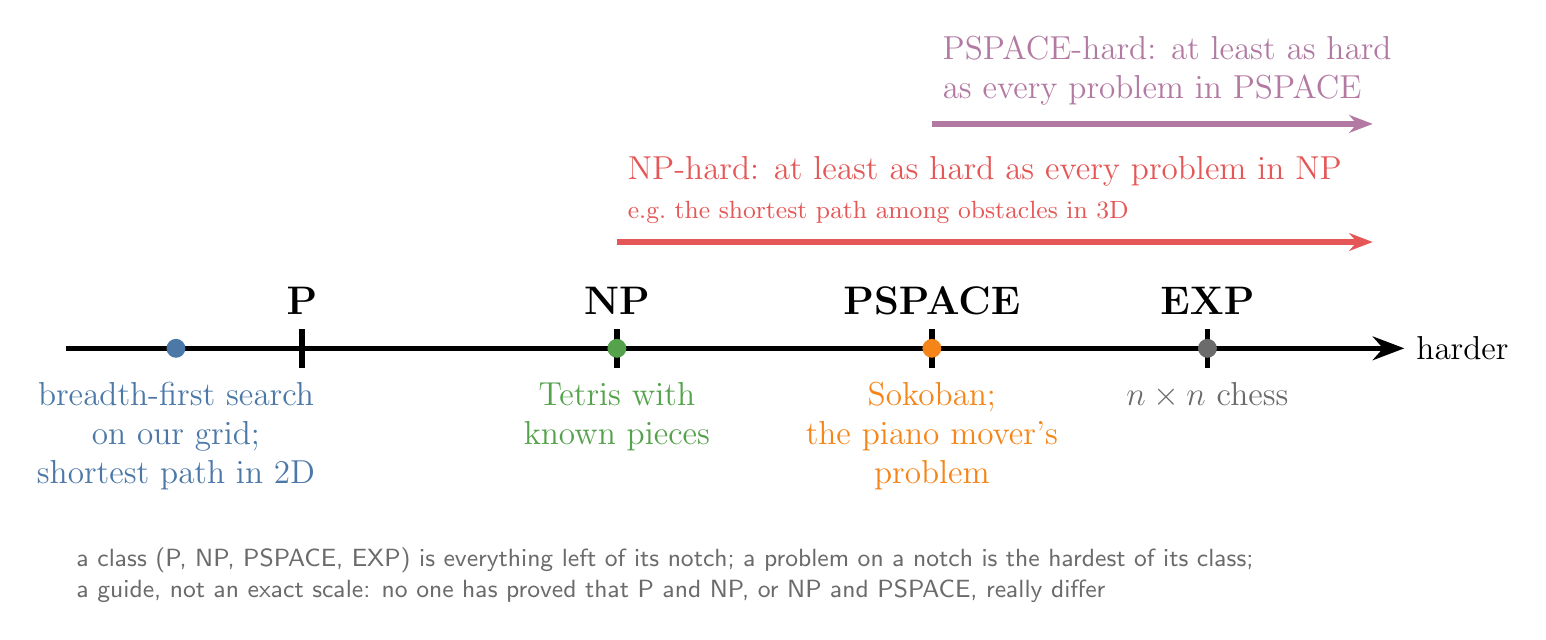
\begin{tikzpicture}[every node/.append style={font=\large}]
  \draw[-{Stealth[length=4mm]}, line width=2pt] (0,0) -- (17,0) node[right, align=left] {harder};
  \foreach \x/\n in {3/P, 7/NP, 11/PSPACE, 14.5/EXP} {
    \draw[line width=2pt] (\x,-0.25) -- (\x,0.25);
    \node[font=\Large\bfseries] at (\x,0.6) {\n};
  }
  % the "-hard" ranges
  \draw[-{Stealth[length=3mm]}, cred, line width=2pt] (7,1.35) -- (16.6,1.35);
  \node[cred, anchor=south west, align=left] at (7,1.45) {NP-hard: at least as hard as every problem in NP\\
    \small e.g.\ the shortest path among obstacles in 3D};
  \draw[-{Stealth[length=3mm]}, cpurple, line width=2pt] (11,2.85) -- (16.6,2.85);
  \node[cpurple, anchor=south west, align=left] at (11,2.95) {PSPACE-hard: at least as hard\\as every problem in PSPACE};
  % examples on the line
  \fill[cblue] (1.4,0) circle (0.12);
  \node[cblue, below, align=center] at (1.4,-0.3) {breadth-first search\\on our grid;\\shortest path in 2D};
  \fill[cgreen] (7,0) circle (0.12);
  \node[cgreen, below, align=center] at (7,-0.3) {Tetris with\\known pieces};
  \fill[corange] (11,0) circle (0.12);
  \node[corange, below, align=center] at (11,-0.3) {Sokoban;\\the piano mover's\\problem};
  \fill[cgrey] (14.5,0) circle (0.12);
  \node[cgrey, below, align=center] at (14.5,-0.3) {$n \times n$ chess};
  \node[note, align=left, anchor=north west] at (0,-2.4) {a class (P, NP, PSPACE, EXP) is everything left of its notch;
    a problem on a notch is the hardest of its class;\\a guide, not an exact scale: no one has proved that P and NP,
    or NP and PSPACE, really differ};
\end{tikzpicture}
\end{document}
